%Edit 0035 ZZZ to report number nnnn 
%Edit 2.4.2 YYMILE to milestone number m.m.m
%Edit Selection of techniques for Uncertainty Quantification YYTITLE to report title - Words Start with Caps
\documentclass[11pt,twoside,a4paper]{article}
%%======================================================================
%% PACKAGES:
%%
%\usepackage{times}               % Times+Helvetica+Courier fonts
\usepackage{helvet}              % helvetica + cmr
\usepackage{fancyhdr}       % package for headers/footers
\usepackage{amsmath}
\usepackage{amssymb}
\usepackage{graphicx}            % Graphics.
%\usepackage{a4}                  % page layout to fit A4
%\usepackage{lastpage}            % get page no of last page
%\usepackage{ifthen}              % logical branching
\usepackage{hyperref}            %insert hyper-links
\usepackage{latexsym}
% uncomment the following to override auto page total
%\pptotal{20}
%%======================================================================

% ensure sans-serif font used throughout
\renewcommand{\familydefault}{\sfdefault}

\newcommand{\culhamissueno}{1.00}%<==edit
\newcommand{\culhamshorttitle}{CD/EXCALIBUR-FMS/0035}%<==edit
\newcommand{\Sec}[1]{Section~\ref{sec:#1}}
\newcommand{\Fig}[1]{Figure~\ref{fig:#1}}
\newcommand{\Tab}[1]{Table~\ref{tab:#1}}
\newcommand{\Eq}[1]{Equation~(\ref{eq:#1})}
\newcommand{\Eqs}[2]{Equations(\ref{eq:#1}) and~(\ref{eq:#2})}
\newcommand{\Figs}[2]{Figures~\ref{fig:#1}--~\ref{fig:#2}}
%Bold lc for script names, tt for computer code and file-names
%\F{NEPTUNE} always in caps
\newcommand{\F}[1]{\textsc{#1}}
\newcommand{\B}[1]{\textbf{#1}}
\newcommand{\T}[1]{{\tt #1}}
\newcommand{\V}[1]{\mathbf{#1}}
\newcommand{\I}[1]{\textit{#1}}
\def\betab{\mbox{\boldmath ${\beta}$}}
\def\lambdab{\mbox{\boldmath ${\lambda}$}}
\newcommand{\nep}{\textsc{NEPTUNE}}
\newcommand{\exc}{\textsc{E}x\textsc{CALIBUR}}
\newcommand{\Papp}{Proxyapp}
\newcommand{\papp}{proxyapp}



%%======================================================================

%% REPORT COVER PAGE Information

\newcommand{\culhamtitle}{\LARGE Selection of techniques for Uncertainty Quantification  \\[1.0\baselineskip] M2.4.2 }%<==edit

%%QA BOX information -- change following as needed
\newcommand{\culhamboardname}{Martin O'Brien}%<==edit
\newcommand{\culhamcontactname}{Rob Akers}%<==edit
\newcommand{\culhamauthor}{Wayne Arter}%<==edit
\newcommand{\culhamauthora}{Ed Threlfall}%<==edit
\newcommand{\culhamauthorb}{Joseph Parker}%<==edit
\newcommand{\culhamauthorc}{Will Saunders}%<==edit
%\newcommand{\culhamcontacttel}{Telephone: 01235 466498}
%\newcommand{\culhamcontactemail}{Email: rob.akers@ukaea.uk}

\newcommand{\culhamdate}{\today}%<=edit
\newcommand{\culhamdatea}{\today}%<=edit
\newcommand{\culhamdateb}{\today}%<=edit

% reproduce Rob's page size

\setlength{\textheight}{220.0mm}
\setlength{\textwidth}{165.0mm}
\setlength{\topmargin}{0.0mm}
\setlength{\oddsidemargin}{0.0mm}
\setlength{\evensidemargin}{\oddsidemargin}
\setlength{\parindent}{0mm}
\addtolength{\parskip}{0.5\baselineskip}
\setlength{\topsep}{0pt}
\setlength{\itemsep}{0pt}

%%======================================================================
\begin{document}

%Titlepage comes out wrong size, but should look right apart from
% picture which cannot be wider than c.150mm.
% To produce conforming report rp1pub.pdf
% remove title page by commenting out lines ending in %<==omit, then
% sed -e '/<==omit$/s/^/%/' < rp1.tex > rp1omit.tex
% pdflatex rp1omit;bibtex rp1omit; pdflatex rp1omit
% pdfunite cover.pdf rp1omit.pdf rp1pub.pdf 
\begin{titlepage}%<==omit
\vspace*{-30mm}%<==omit

\includegraphics[width=2.5cm]{../corpics/cofaplus} \\[2.0\baselineskip]%<==omit
{\LARGE {\textbf{\textsf{ExCALIBUR}}}}\\[2.0\baselineskip]%<==omit
{\LARGE \culhamtitle } \\[2.0\baselineskip]%<==omit
{\textbf{\textsf{Abstract}}}\\%<==omit
The report describes work for \exc \ project \nep \ %<==omit
at Milestone 2.4.2. %<==omit
Report on UQ selection.
%<==omit
%<==omit
\vfill%<==omit
\centerline{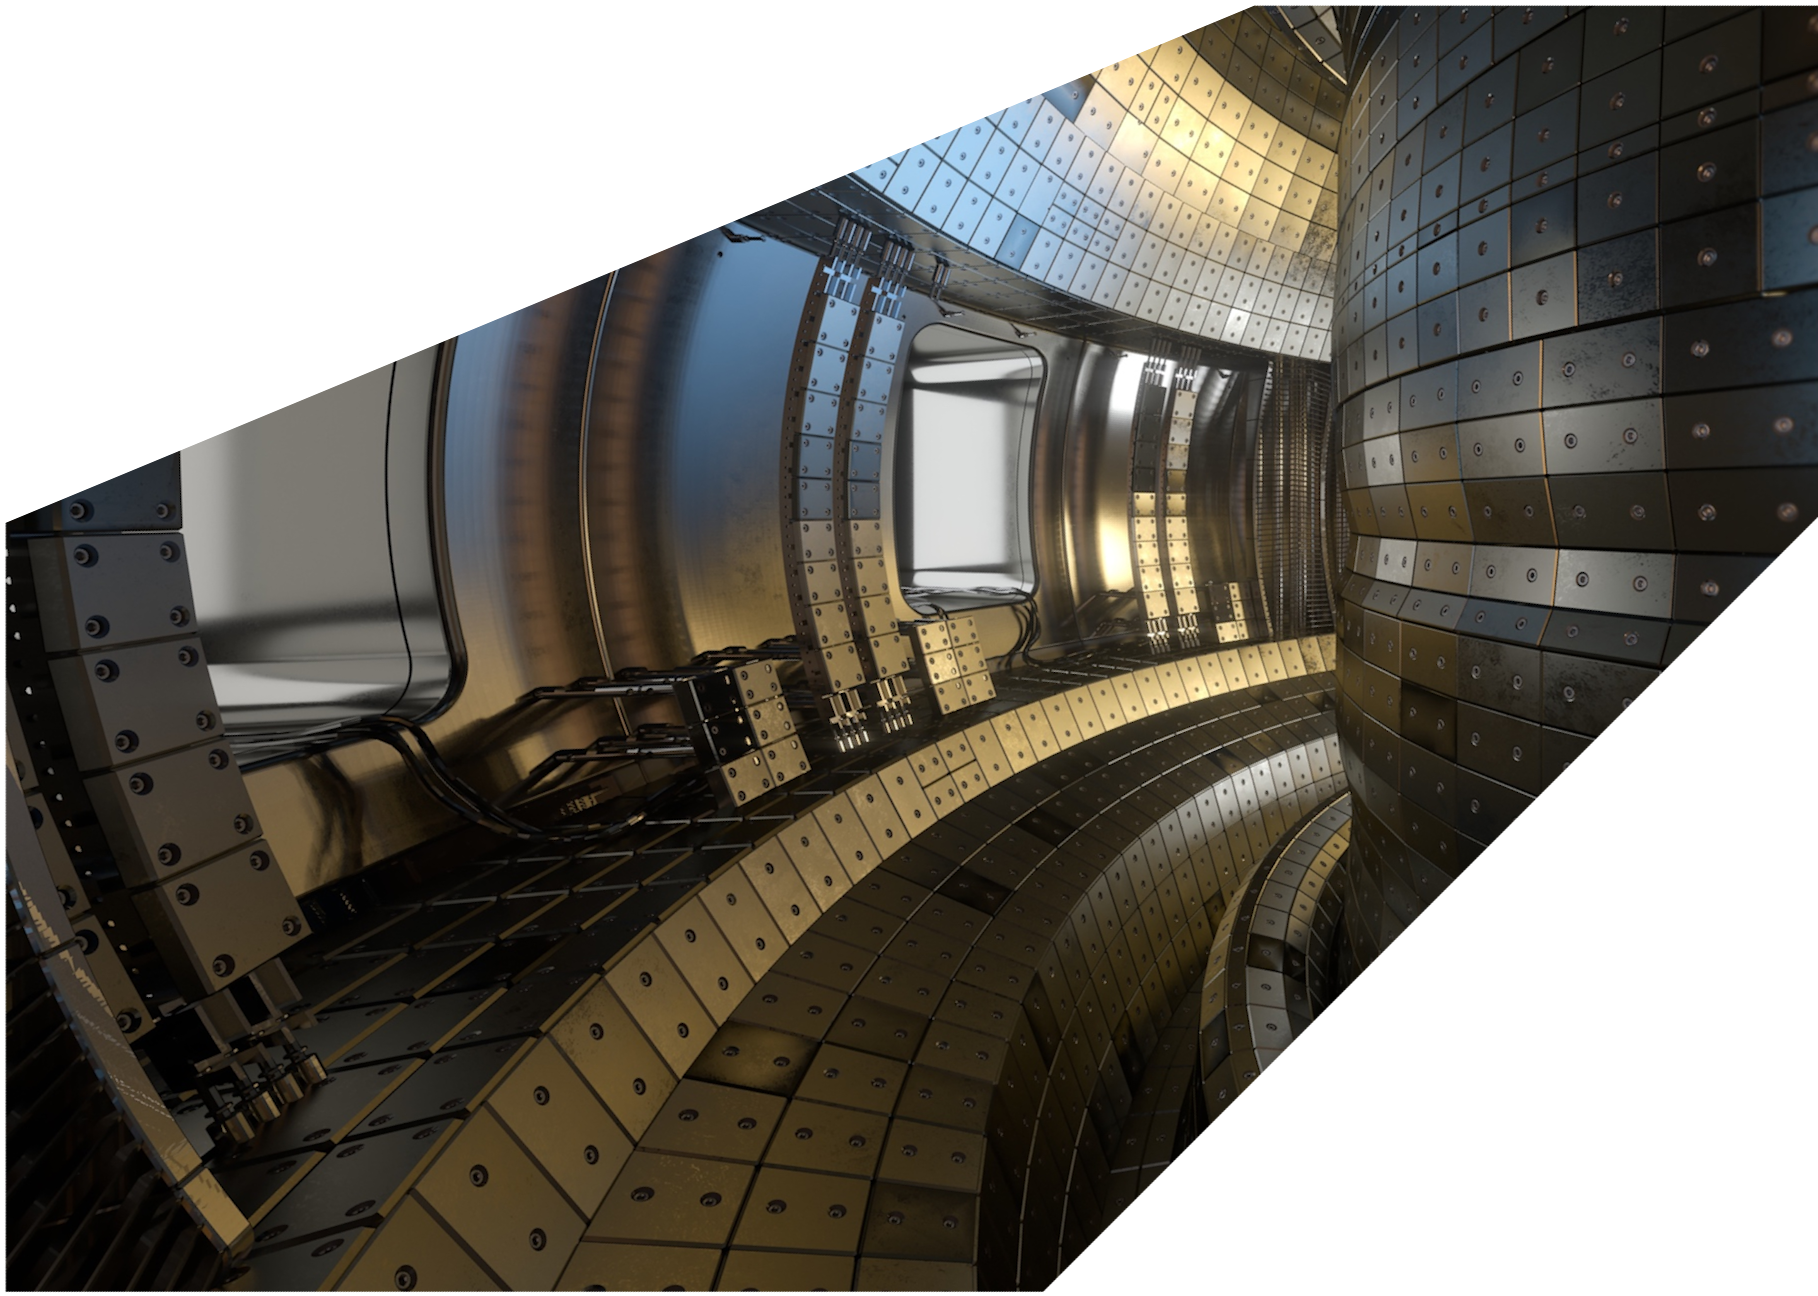
\includegraphics[width=0.9\textwidth]{../corpics/tokintcrop}}%<==omit
\end{titlepage}%<==omit

\hspace{-30mm}\begin{table}[h]
\sffamily
\begin{center}
\textbf{\textsf{UKAEA REFERENCE AND APPROVAL SHEET}}
\begin{tabular}{||p{5.7cm}|p{4.7cm}|p{5.0cm}||}
\hline
\hline
& Client Reference: &  \\
\hline
& UKAEA Reference: & \culhamshorttitle \\
& & \\
\hline
& Issue: & \culhamissueno \\
\hline
& Date: & \culhamdateb \\
\hline
\multicolumn{3}{||l||}{} \\
\multicolumn{3}{||l||}{Project Name: ExCALIBUR Fusion Modelling System} \\
\multicolumn{3}{||l||}{} \\
\hline
\end{tabular}
\begin{tabular}{||p{3.3cm}|p{4.6cm}|p{3.5cm}|p{3.6cm}||}
\hline
& Name and Department & Signature & Date \\
\hline
Prepared By: & \culhamauthor & N/A & \culhamdate \\
& \culhamauthora & N/A & \culhamdate \\
& \culhamauthorb  & N/A & \culhamdate \\
& \culhamauthorc  & N/A & \culhamdatea \\
& & & \\
& BD & & \\
\hline
Reviewed By: & \culhamcontactname & 
\includegraphics[width=3.0cm]{../corpics/blanksign}& \culhamdatea \\
& & & \\
& Advanced Computing Dept. Manager & & \\
\hline
Approved By: & \culhamboardname  & 
\includegraphics[width=3.0cm]{../corpics/blanksign} & \culhamdateb \\
& & & \\
& MSSC & &\\
\hline
\hline
\end{tabular}
\end{center}
\end{table}


\clearpage
\subsection{GP vs NN}\label{sec:gpvsnn}
Both basically very expensive techniques for interpolation
\begin{enumerate}
\item GP 
\begin{enumerate}
\item At each position/time$x$ there is a Gaussian random variable. However
\item the correlation between different $x$ need not be Gaussian, and 
\item the correlation function $R(x,x')$ essentially defines how the interpolant is produced, at $N^3$ cost, $N$ is number of samples.
\item The correlation function has (hyper)parameters which may be calculated by optimisation - maximising the likelihood function over relatively small number of parameters, but optimiser may not converge
\item May do amazingly well as a consequence of the Central Limit Theorem
\item Likely to be stable when extrapolating if $R$ smooth
\end{enumerate}
\item NN
\begin{enumerate}
\item Defined by localised functions at nodes
\item Fitting by optimisation techniques for number of parameters $\propto$ number of nodes - techniques rely on having many samples and optimiser may be slow to converge or overfit
\item Theorems that NN approximation has resistance to ``curse of dimensionality"
\item Usually unstable when extrapolating
\end{enumerate}
\end{enumerate}

\subsection{GP}\label{sec:gp}
Fundamentally the Gaussian Process~(GP) is a stochastic interpolant between the
sample data points. The wikipedia entry~\cite{krigingwiki} helpfully shows that for
Gaussian statistics, the GP amounts to a Brownian walk which takes in the sample
points in turn. It will be seen why there is an optimal MSE, in that if the amplitude
of the walk is too small,
then the interpolant will fail to change enough to go through consecutive points that have
very different sample values,  too large an MSE
and it is becomes increasingly improbable that the walk will `hit' the points.
It also follows that it is vital to accurately characterise the statistics of
the stochastic process as they are integral to the interpolation.
Ordinary Kriging assumes that the data has a constant mean at least locally.
There follows a description of universal Kriging that tries to fit a
combination of stochastic function and a deterministic functional
form (typically a polynomial) through the sample point.

The most comprehensive  work appears to be Sacks~et~al~\cite{Sa89Desi}, who 
suppose that, although the system under is deterministic (so that its output~$y$
at a sample point~$x$ should always be the same), because of errors $y(x)$  can be 
regarded as resulting from a random function \emph{aka} stochastic process
as follows:
\begin{equation}\label{eq:ystoc}
Y(x)= \Sigma^M_{m=1} c_m f_m(x) + Z(x) = {\mathbf c}\cdot {\bf f}(x) + Z(x)
\end{equation}
where the $f_m(x)$~are a basis that may be chosen by the modeller, $c_m$ are
fitting parameters to be determined, and $Z(x)$~is a (separate) random process at every~$x$
with zero expected value. The assumption represented by \Eq{ystoc} is referred to as universal Kriging,
distinguishing it from the simple Kriging described in ref~\cite[\S\,2.3.1]{y2re313}.
Further suppose that the experimental design, ie.\ the set of samples, is
\begin{equation}
\mbox{Experimental design}\;\;{\bf S}=(x_1,x_2,\ldots,x_N)
\end{equation}
leading to observed values ${\bf y}=\left(y(x_1),y(x_2),\ldots,y(x_N)\right)$. If~${\bf y}$
is all the information known about the system, then it is reasonable further to
suppose that an any point~$x$, $y(x)$ may be predicted as a linear combination of
the observations
\begin{equation}
\tilde{y}(x)=\betab(x)\cdot{\bf y} 
\end{equation}
where the $N$-vector of coefficients $\betab(x)$ is chosen to minimise the mean square-error
\begin{equation}\label{eq:mse}
MSE\left(\tilde{y}(x)\right) = \mathbb{E} [ \left( \betab(x)\cdot{\bf y} - Y(x) \right)^2 ]
\end{equation}
subject to the constraint
\begin{equation}\label{eq:nobias}
\mathbb{E} [ \left( \betab(x)\cdot{\bf y} - Y(x) \right) ] = 0
\end{equation}
Substituting \Eq{ystoc} in the argument of \Eq{nobias} gives
\begin{equation}
\betab(x)\cdot{\bf y} - Y(x)  = \Sigma^N_{n=1} \beta_n(x)\left({\mathbf c}\cdot {\bf f}(x_n) + Z(x_n)\right)
-\left( {\mathbf c}\cdot {\bf f}(x) + Z(x) \right)
\end{equation}
giving
\begin{equation}
\mathbb{E} [ \left( \betab(x)\cdot{\bf y} - Y(x) \right) ] = 
\mathbb{E} [ {\mathbf c}\cdot  \Sigma^N_{n=1}\left(\beta_n(x) {\bf f}(x_n) - {\bf f}(x) \right) ]
\end{equation}
since $\mathbb{E} [ Z(x) ] = 0$ at each value of~$x$. Thus the constraint \Eq{nobias} implies
\begin{equation}\label{eq:fseqf}
\Sigma^N_{n=1}\beta_n(x) {\bf f}(x_n) = {\bf f}(x)
\end{equation}
which may be written in matrix-vector form as
\begin{equation}\label{eq:consm}
F^T \betab(x) = {\bf f}(x)
\end{equation} 
where the size~$N \times M$ matrix
\begin{equation}
F = \begin{pmatrix}
f_1(x_1) & f_2(x_1) & \ldots & f_M(x_1) \\
f_1(x_2) & f_2(x_2) & \ldots & f_M(x_2) \\
& & \ldots & \\
f_1(x_N) & f_2(x_N) & \ldots & f_M(x_N) 
\end{pmatrix}
\end{equation}
 
Substituting \Eq{fseqf} in $\left( \betab(x)\cdot{\bf y} - Y(x) \right)^2$, all that remains are the
terms in~$Z$, so
\begin{eqnarray}
MSE\left(\tilde{y}(x)\right) &=& \mathbb{E} [ \left( \Sigma^n_{s=1} \beta_s(x) Z(x_s) - Z(x) \right)^2 ] \\
&=& \mathbb{E} [ \left( \Sigma^n_{s=1} \beta_s(x) Z(x_s) . \Sigma^n_{q=1} \beta_q(x) Z(x_q) -2 \Sigma^n_{s=1} \beta_s(x) Z(x_s) . Z(x) + Z(x)^2 \right) ] 
\end{eqnarray}
Define the (normalised) correlation matrix by
\begin{equation}
\mathbb{E} [ Z(x_i) Z(x_j) ]= \sigma^2 R(x_i,x_j) 
\end{equation}
so that its entries~$R_{ij}$ are symmetric by construction, and the vector
\begin{equation}
{\bf r}(x)=\left( R(x_1,x), R(x_2,x),\ldots,R(x_n,x) \right)
\end{equation}
then
\begin{equation}\label{eq:msend}
MSE\left(\tilde{y}(x)\right) = \sigma^2\left(1+ \betab(x) R \betab(x) - 2 \betab(x)\cdot{\bf r}(x) \right) 
\end{equation}
which must be a minimum as a function(al) of~$\betab$ subject to the constraint system~\Eq{consm}.
Introducing $\lambdab(x)$ as a $M$-vector of Lagrange multipliers corresponding to the constraint,
it follows (since varying \Eq{consm} gives rise simply to a term $F^T$) that
\begin{equation}\label{eq:mat2}
R \betab(x) -{\bf r}(x) + F \lambdab(x)=0
\end{equation}
thus to obtain $\betab(x)$ requires solving the coupled system
\begin{equation}\label{eq:endsm}
\begin{pmatrix}
0 & F^T \\
F & R
\end{pmatrix}
\begin{pmatrix}
\lambdab(x) \\
\betab(x)
\end{pmatrix}
=
\begin{pmatrix}
{\bf f}(x) \\
{\bf r}(x)
\end{pmatrix}
\end{equation}
which it is convenient to rearrange as
\begin{equation}\label{eq:endsmt}
\begin{pmatrix}
R & F \\
F^T & 0
\end{pmatrix}
\begin{pmatrix}
\betab(x) \\
\lambdab(x)
\end{pmatrix}
=
\begin{pmatrix}
{\bf r}(x) \\
{\bf f}(x)
\end{pmatrix}
\end{equation}
and once a solution $(\betab(x), \lambdab(x))$ has been obtained then substituting for $R \betab$
from \Eq{mat2} in \Eq{msend} and using \Eq{consm} gives
\begin{equation}\label{eq:msendsub}
MSE\left(\tilde{y}(x)\right) = \sigma^2\left(1 - \betab(x) \cdot{\bf r}(x) - \lambdab(x) \cdot{\bf f}(x) \right) 
\end{equation}

The theory of block matrices in \Sec{matrixth} specifically \Eq{matrixth0}, gives the solution to \Eq{endsmt}
in terms of a negative inverse Schur complement $S = -S_C^{-1} = (F^TR^{-1}F)^{-1}$ as
\begin{equation}\label{eq:endsol}
\begin{pmatrix}
\betab(x) \\
\lambdab(x)
\end{pmatrix}
=
\begin{pmatrix}
R^{-1} - R^{-1}FSF^T R^{-1} & R^{-1} FS \\
SF^TR^{-1} & -S
\end{pmatrix}
\begin{pmatrix}
{\bf r}(x) \\
{\bf f}(x)
\end{pmatrix}
=
\begin{pmatrix}
R^{-1} - F^{+T}S^{-1}F^+ &  F^{+T}\\
F^+ & -S
\end{pmatrix}
\begin{pmatrix}
{\bf r}(x) \\
{\bf f}(x)
\end{pmatrix}
\end{equation}
where the right pseudo-inverse of~$F$, $F^+=SF^TR^{-1}$ (note $SF^TR^{-1}. F = I$) has been inroduced.
It is also worth noting that $S$~only exists if $N\geq M$ and it is then symmetric.

The formulae in the Sacks~et~al paper then follow from the solution
\begin{eqnarray}\label{eq:betasol}
\betab(x) &=& (I - R^{-1}FSF^T) R^{-1} {\bf r} +R^{-1} FS {\bf f}  = (R^{-1} - F^{+T}S^{-1}F^+) {\bf r} + F^{+T} {\bf f} \\  
\lambdab(x) &=& SF^TR^{-1} {\bf r} -S {\bf f} = F^+ {\bf r} -S {\bf f} \label{eq:lambdasol}
\end{eqnarray}
upon introducing
\begin{equation}\label{eq:ctilde}
{\bf \tilde{c}}= SF^TR^{-1}{\bf y} = F^+ {\bf y}
\end{equation}
and using the fact that for a general matrix~$F$ is symmetric, then for arbitrary vectors ${\bf x}$
and ${\bf z}$, $F^T {\bf x} \cdot {\bf z}= {\bf x} \cdot F {\bf z} = {\bf x} F {\bf z}$, so that
\Eq{betasol}  yields
\begin{equation}\label{eq:ytilde}
\tilde{y}= \betab \cdot {\bf y} = {\bf \tilde{c}} \cdot {\bf f} +
  R^{-1} {\bf r} \cdot ({\bf y}-F {\bf \tilde{c}})
\end{equation}
Setting ${\bf \tilde{c}}= {\bf 0}$ recovers simple Kriging.
 
Another  formula is
\begin{equation}\label{eq:msendsubf}
MSE\left(\tilde{y}(x)\right) = \sigma^2\left(1 - {\bf r}(R^{-1} - F^{+T}S^{-1}F^+){\bf r} 
-2 {\bf r} F^+ {\bf f} + {\bf f}S{\bf f} \right) 
\end{equation}

\section{Matrix Theory}\label{sec:matrixth}
\subsection{Key Results}\label{sec:mthkey}
The inverse of a block matrix, ie.\ a matrix written as
\begin{equation}\label{eq:blkmat}
B=\begin{pmatrix}
A_{11} & A_{12} \\
A_{21} & A_{22}
\end{pmatrix}
\;\;\mbox{structure}\;\;
\begin{pmatrix}
N \times N & N \times M \\
M \times N & M \times M
\end{pmatrix}
\end{equation}
may be deduced from the formulae obtained using Gaussian elimination for
$2$~simultaneous linear equations (expressed using  the $2 \times 2$~matrix~$A$)
%\begin{pmatrix}
%a_{11} & a_{12} \\
%a_{21} & a_{22}
%\end{pmatrix}
\begin{equation}
A
\begin{pmatrix}
x \\
y
\end{pmatrix}
=
\begin{pmatrix}
b_1 \\
b_2
\end{pmatrix}
\;\;\mbox{where} \;\;
A=
\begin{pmatrix}
a_{11} & a_{12} \\
a_{21} & a_{22}
\end{pmatrix}
\end{equation}
As is well-known, Gaussian elimination proceeds by scaling the $x$-coefficient of the
first equation to be equal to that~$a_{21}$ of the second, ie.\ by the factor $a_{21} a_{11}^{-1}$
and then subtracting the two equations. This may be expressed as a matrix multiply, viz.
\begin{equation}
\begin{pmatrix}
1 & 0 \\
-a_{21} a_{11}^{-1} & 1
\end{pmatrix}
\begin{pmatrix}
a_{11} & a_{12} \\
a_{21} & a_{22}
\end{pmatrix}
=
\begin{pmatrix}
a_{11} & a_{12} \\
0 & s_c
\end{pmatrix}
\end{equation}
where the coefficient 
\begin{equation}\label{eq:scaschur}
s_c=a_{22} - a_{21} a_{11}^{-1} a_{12}
\end{equation}
It follows that the inverse of~$A$, provided $s_c\neq0$  is
\begin{equation}\label{eq:sinv3fac}
A^{-1}=
\begin{pmatrix}
1 & a_{21}^{-1} a_{12} \\
0 & 1
\end{pmatrix}
\begin{pmatrix}
a_{11}^{-1} & 0 \\
0 & s_c^{-1}
\end{pmatrix}
\begin{pmatrix}
1 & 0 \\
-a_{21} a_{11}^{-1} & 1
\end{pmatrix}
\end{equation}


The Schur complement is the analogue of the~$s_c$ factor for block matrices, viz.
\begin{equation}\label{eq:schur}
S_C=A_{22} - A_{21} A_{11}^{-1} A_{12}
\end{equation}
when writing \Eq{sinv3fac} with $a_{ij}\rightarrow A_{ij}$ ($s_c\rightarrow S_C$, invertible) gives 
the block factorisation. Multiplying out the product gives
\begin{equation}\label{eq:matrixth0}
B^{-1}=
\begin{pmatrix}
A_{11}^{-1} 
+A_{11}^{-1}A_{12}S_C^{-1}A_{21}A_{11}^{-1} & -A_{11}^{-1}A_{12}S_C^{-1} \\
-S_C^{-1}A_{21}A_{11}^{-1} & S_C^{-1}
\end{pmatrix}
\end{equation}

\subsection{Additional Results}\label{sec:mthadd}
Using the generalised Sherman-Morrison-Woodbury formula, the first entry simplifies. The formula, from
Golub \& van Loan~\cite[Eq.\,(2.1.4)]{golubvanloan} is
\begin{equation}\label{eq:smw}
(T+UV)^{-1}=T^{-1}-T^{-1}U(I+VT^{-1}U)^{-1}VT^{-1}
\end{equation}
where $T$ is an $N \times N$~matrix, $U$ is $N \times M$ and $V$ is~$M \times N$
(cf.\ use of $V^T$ in~\cite{golubvanloan}).
To apply, write $U=-WC^{-1}$, then
\begin{equation}\label{eq:smwp}
(T-WC^{-1}V)^{-1}=T^{-1}+T^{-1}W \left[C^{-1}(I-VT^{-1}WC^{-1})^{-1}\right] VT^{-1}
\end{equation}
and observe that the term is square brackets simplifies on remembering that 
where inverses of matrices~$S_j$ exist, $S_1^{-1}S_2^{-1}= (S_2 S_1)^{-1}$, so that
\begin{equation}\label{eq:smwq}
(T-WC^{-1}V)^{-1}=T^{-1}+T^{-1}W \left[C-VT^{-1}W)\right]^{-1} VT^{-1}
\end{equation}
With the obvious substitutions, this implies
\begin{equation}\label{eq:smw2}
(A_{11}-A_{12}A_{22}^{-1}A_{21})^{-1}=A_{11}^{-1}+A_{11}^{-1}A_{12}[S_C]^{-1}A_{21}A_{11}^{-1}
\end{equation}
Thus 
\begin{equation}\label{eq:matrixth}
B^{-1}=
\begin{pmatrix}
(A_{11}-A_{12}A_{22}^{-1}A_{21})^{-1} & -A_{11}^{-1}A_{12}S_C^{-1} \\
-S_C^{-1}A_{21}A_{11}^{-1} & S_C^{-1}
\end{pmatrix}
\end{equation}


There are results of the form
\begin{equation}\label{eq:invprod}
(T-UV^{-1}W)^{-1}UV^{-1}=T^{-1}U(V-WT^{-1}U)^{-1}
\end{equation}
perhaps more memorable as
\begin{equation}\label{eq:invinvprod}
(T^{-1}-UVW)^{-1}UV^{-1}=TU(V^{-1}-WTU)^{-1}
\end{equation}
These are easily proven by multiplication by the terms in parenthesis, when (in the
second case \Eq{invinvprod}, two terms in $UVWTU$  cancel. The importance
of \Eq{invprod} is that the off-diagonal terms in~$S_C^{-1}$ in \Eq{matrixth}
may be replaced by terms expressed using $(A_{11}-A_{12}A_{22}^{-1}A_{21})^{-1}$.

\clearpage
\section*{Acknowledgement}\label{sec:ackn}
\emph{The support of the UK Meteorological Office and Strategic Priorities Fund is acknowledged.}


%\section*{References}
\bibliographystyle{unsrt}
\bibliography{../bib/new,../bib/waynes,../bib/misc,../bib/warv,../bib/neuts,../bib/reac,../bib/exc,../bib/active,../bib/dg1srt}

\end{document}
